\documentclass[16pt,a4paper]{article}

\usepackage{fontspec}
\setmainfont[BoldFont=黑体]{方正新书宋简体}          
\XeTeXlinebreaklocale "zh"                    
\XeTeXlinebreakskip = 0pt plus 1pt minus 0.1pt  

\usepackage{indentfirst} 
\setlength{\parindent}{2em}

\usepackage{changepage}
\usepackage{float}
\usepackage{setspace}
\usepackage{amsmath}
\usepackage{amsfonts}
\usepackage{amssymb}

\usepackage{geometry}
\geometry{left=2.5cm,right=2.5cm,top=2.5cm,bottom=4cm}
\usepackage{fancyhdr}
\pagestyle{fancy}
\lhead{\includegraphics[scale=0.5]{logo.png}}

\author{郭嘉丞 \quad 姚皓天}
\title{数字听诊器 \\ Digital Stethoscope}
\date{2015年6月}

\graphicspath{{Figure/}}

\begin{document}
\maketitle
\thispagestyle{empty}
\newpage
\section{简介}

\section{系统设计}


\section{硬件设计细节}
\subsection{电源部分}
电源是系统中容易被忽视,但是又非常重要关乎系统性能的关键部分。\\
本设计中含有数字部分和模拟部分,各自使用独立的电源:
\begin{itemize}
\item 数字部分采用 Step-Down(Buck) Converter
\item 模拟部分采用 High PSRR, Low Noise, Single Output LDO
\end{itemize}

\subsubsection{数字电源}
\begin{figure}[H]
\centering
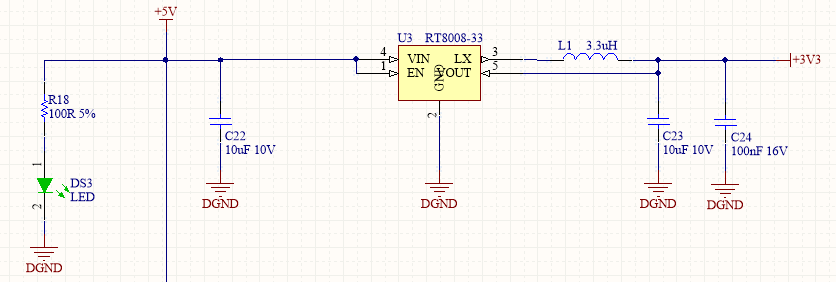
\includegraphics[width=0.8\textwidth]{power1.png}
\caption{开关电源} 
\end{figure}
数字部分采用Richtek RT8008-3.3供电。这款芯片具有以下特点:
\begin{enumerate}
\item 固定输出电压3.3V
\item 1.5MHz的PWM频率,可以使用小型的外部电感和电容
\item 内置场效应管,采用同步整流方式,具有较高的效率
\end{enumerate}\par
由于具有效率高,体积小,占用PCB面积小的特点,非常适合为本设计的数字部分供电,也利于手持设备小型化。\par
图中DS3用作电源指示灯。

\subsubsection{模拟电源}
\begin{figure}[H]
\centering
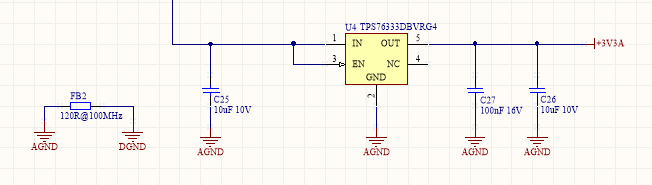
\includegraphics[width=0.8\textwidth]{power2.png}
\caption{线性电源} 
\end{figure}
模拟部分采用TI TPS79333供电。这款芯片具有以下特点:

\begin{enumerate}
\item 高PSRR(70 dB at 10 kHz)
\item 低噪声(32 $\mu V_{RMS}$)
\end{enumerate}\par
该芯片可以有效抑制电源噪声,提供符合模拟部分工作的低噪声电源。\par
图中FB2 采用120R@100MHz的磁珠将模拟地与数字地相连,可以避免数字部分对模拟部分的干扰。
\subsection{模拟前端和数据转换}
模拟前端和数据转换采用TI Audio Codec TLV320AIC23B为核心,辅以外部电路,实现声音信号和数字信号的双向转换。
\subsubsection{话筒输入}
\begin{figure}[H]
\centering
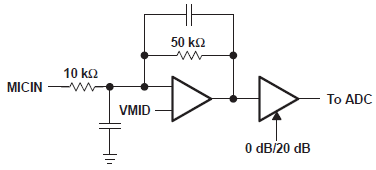
\includegraphics[scale = 1]{Mic1.png}
\caption{话筒输入电路} 
\end{figure}

\begin{figure}[H]
\centering
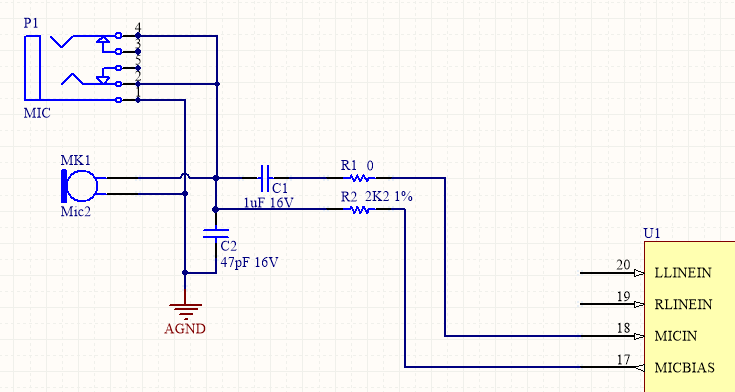
\includegraphics[width=0.8\textwidth]{Mic2.png}
\caption{话筒输入电路} 
\end{figure}

芯片输出话筒偏置电压,经R2供给话筒。话筒将声音转换为变化的电压,经C1耦合输入CODEC。通过调节R2可以调节输入信号的第一级放大增益。

\subsubsection{耳机输出}
\begin{figure}[H]
\centering
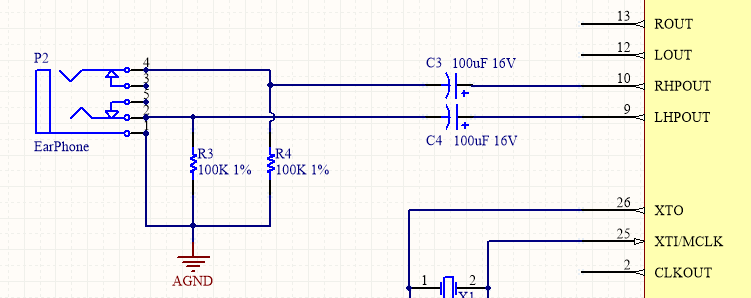
\includegraphics[width=0.8\textwidth]{EarPhone.png}
\caption{耳机输出电路} 
\end{figure}
由于芯片内置耳放,所以输出信号的左右声道分别直接通过C3和C4耦合至耳机输出即可。

\subsubsection{CODEC的数字接口}
\begin{figure}[H]
\centering
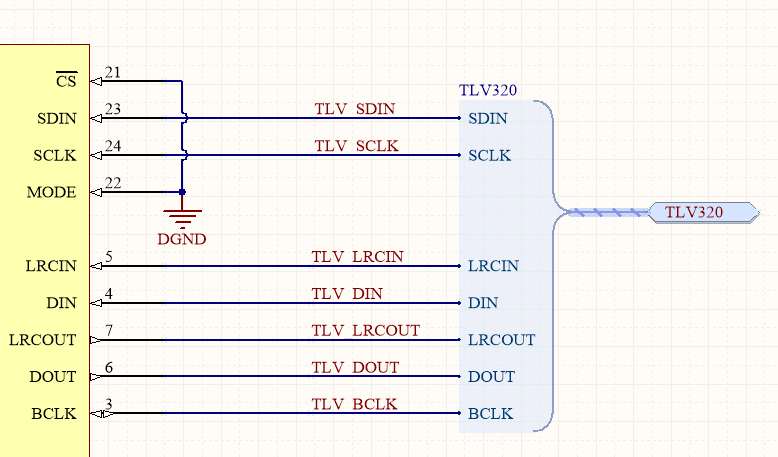
\includegraphics[width=0.8\textwidth]{DI.png}
\caption{CODEC的数字接口} 
\end{figure}
CODEC与MCU之间通过数字接口相连。控制接口为I2C接口,用于配置COEDC的输入输出方式,可编程放大器的放大增益,信号流向等。音频数据采用I2S接口相连。

\subsection{微控制器和其他数字外设}
\subsubsection{微控制器}
微控制器采用NXP LCP1768。微控制器为ARM Cortex-M3内核。
\begin{figure}[H]
\centering
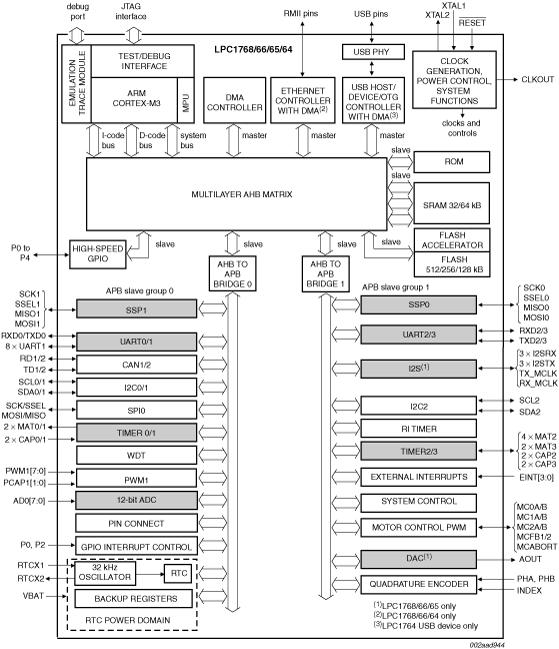
\includegraphics[width=0.7\textwidth]{LPC1768.png}
\caption{LPC1768内部框图} 
\end{figure}

\subsubsection{TF-Card}
\begin{figure}[H]
\centering
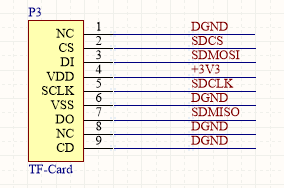
\includegraphics[scale = 0.8]{TF-Card.png}
\caption{TF-Card} 
\end{figure}

\subsubsection{USB接口}
\begin{figure}[H]
\centering
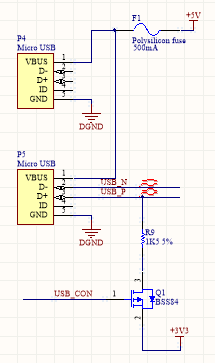
\includegraphics[scale = 1]{USB.png}
\caption{USB接口} 
\end{figure}

P4接口用于给系统供电,电源入口串有多晶硅熔丝,用于对系统和外部电源的保护。P5接口用于接驳其他的USB外部设备(如U盘)或者连接个人计算机。

\subsubsection{调试接口}
\begin{figure}[H]
\centering
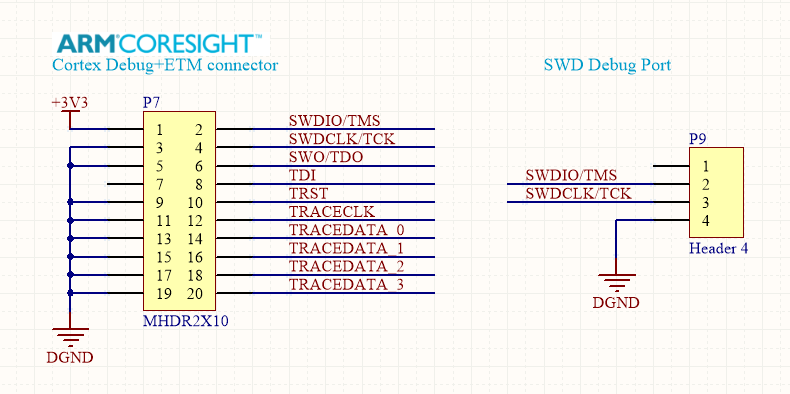
\includegraphics[width=0.6\textwidth]{debug.png}
\caption{调试接口} 
\end{figure}
留有两种调试接口。其中SWD Debug Port可以连接通用的调试工具。而标准的Cortex Debug+ETM connector可以用于连接ARM U-Link Pro等带有Trace功能的调试工具,提供更加丰富的调试功能。

\subsubsection{其他外设}
\begin{figure}[H]
\centering
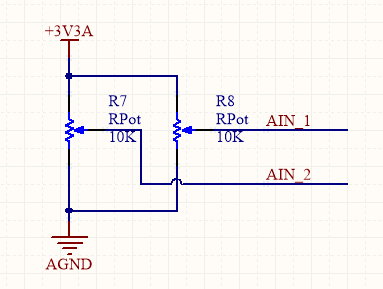
\includegraphics[scale = 0.8]{Rpot.png}
\caption{旋钮} 
\end{figure}


\begin{figure}[H]
\centering
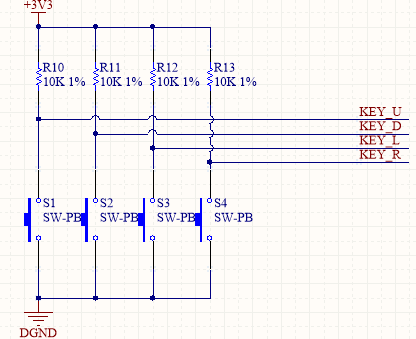
\includegraphics[scale = 0.8]{key.png}
\caption{按键} 
\end{figure}

\begin{figure}[H]
\centering
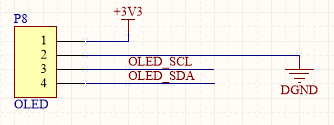
\includegraphics[scale = 0.8]{oled.png}
\caption{OLED屏幕} 
\end{figure}

这些外设可以用于扩展功能。

\section{PCB设计}
\begin{figure}[H]
\centering
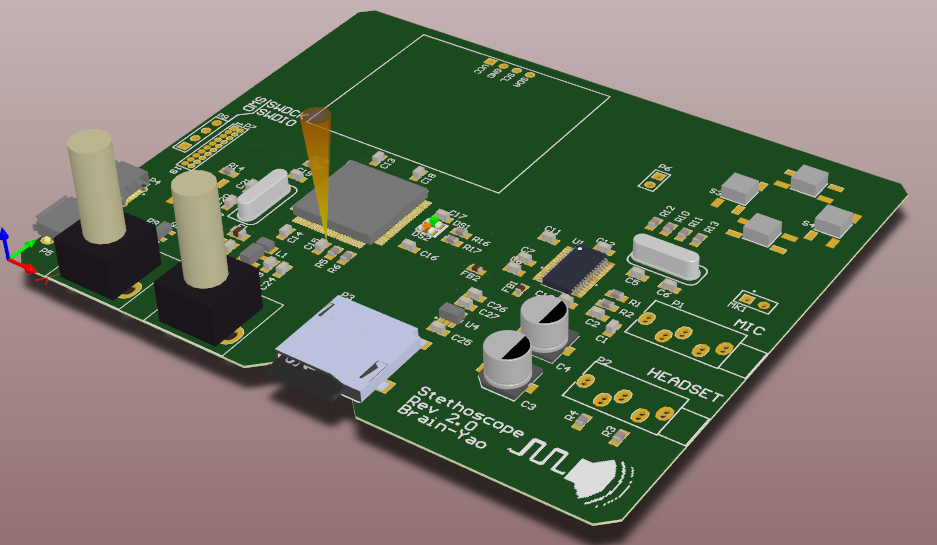
\includegraphics[width=0.8\textwidth]{pcb3D.png}
\caption{PCB三维渲染图} 
\end{figure}
PCB设计采用Altium Designer 设计,按照通常混合信号系统的设计方法,数模部分分开布局。数字地、模拟地按布局切分,单点相连。


\section{软件设计}

\section{开发时间节点}

\section{测试效果}

\section{项目总结}
\end{document}
